\section{From Instrumentation to Completion Deadlines}
\label{app:deadline-study}

The preceding experiment isolates a certification capability, but its two
duration limits produce the same completion counts. We now separate a system
limit that we can attain exactly from the performance of a practical
multidimensional controller. The first study implements the existing scalar
Gaussian theorem. The second uses the unchanged bounded-report verifier,
crosses both stage-counter orientations, and includes empty history. These
studies have separately frozen protocols and new evaluation seeds. Neither
converts abstract acquisition units into a measured physical deadline.

\subsection{An Exact Instrument and Resource Benchmark}

A cheaper service has radio mean $6+\vartheta$, server mean
$6-\vartheta$, and total mean $12$. Its limits are $6$, $7$, and $13$,
respectively. A known-safe backup has a higher charge beyond the optimality
tolerance. On the continuous class
$\vartheta\in(-0.8,0.8)\setminus\{0\}$, the cheaper service is the unique
valid answer for negative $\vartheta$; the backup is the unique valid answer
for positive $\vartheta$. The server and total constraints are nonbinding
in this deliberately scalar reference problem.

Centered aggregate, radio, and server reports have Gaussian means
$0$, $\vartheta$, and $-\vartheta$. The report errors are independent, with
known variances. Gaussianity describes the diagnostic reports, not packet
latency. Aggregate observations contain no information about the answer.
We compare aggregate-only access, either counter separately, and both
counters. There is no history.

Radio and server reports cost 1 and 6 units and take 1 and 4 serialized
duration units. One catalogue gives them variances $1$ and $1/9$; the other
reverses those variances. The acquisition-cost cap and each count cap are
512. We compute designs for every integer deadline $H=0,\ldots,512$.
This fixed catalogue deliberately changes which counter supplies the most
information per unit time or expenditure.

Let $A_{\max}(H)$ denote the maximum attainable precision under these exact
integer constraints. An integer dynamic program selects the design using
only the public measurement operators, variances, costs, durations, and caps.
It never receives $\vartheta$. Theorem~\ref{thm:scalar-deadline} gives
$$
P^\star(H,\vartheta)
 =\Phi\!\left(|\vartheta|\sqrt{A_{\max}(H)}-z_{0.95}\right).
$$
Thus 95\% correct completion is attainable precisely when
$$
|\vartheta|\sqrt{A_{\max}(H)}\geq2z_{0.95}.
$$
The unknown margin enters this capability assessment, not the executable
design. The controller cannot advertise a per-request 95\% completion
promise from the evaluator's margin. A completion requirement over a class
of operating instances instead needs a stated minimum nonzero margin. No finite resource
budget gives a completion level above the risk allowance uniformly over
arbitrarily small margins.

We implement the maximizing design and its endpoint test: return the
positive or negative answer if the standardized score exceeds $z_{0.95}$
or falls below $-z_{0.95}$; otherwise return unresolved. The design and test
attain the frontier simultaneously for every nonzero margin when precision
is positive. At zero precision, the theoretical 0.05 frontier permits
data-free randomized answers. Our operational implementation always
abstains instead; we keep this deliberate non-attainment case explicit.

\subsection{Early Decisions and the Meaning of the Limit}

A second policy uses the same fixed integer design but checks after every
returned report. It orders reports by known precision per duration. For
$N>1$ reports, intermediate check $j<N$ receives one-sided risk
$0.01/[j(j+1)]$, and the final check receives $0.04$. A one-report design
uses $0.05$ at its only check. At a fixed nonzero margin, only the opposite
sign is wrong, so the union bound controls wrong returns by $0.05$.
We do not repeatedly apply the fixed-endpoint threshold under optional
stopping. Only the currently requested report values enter the policy.

This early-stopping policy may save acquisition cost or return sooner while
reducing correct completion. The exact theorem optimizes correct completion
under hard resources; it does not say that the endpoint design minimizes
expected stopped cost. Each deadline defines a separately specified policy,
not a license to reset risk when extending an ongoing request.

We evaluate margins $\pm0.1$, $\pm0.2$, and $\pm0.4$ at deadlines
$0$, $8$, $32$, $128$, and $512$. Each of the 480 policy/condition cells
uses 4096 independent seeds. Standardized innovations are paired across
policies and conditions; they are not additional independent replications.
The 1,966,080 recorded outcomes retain correct, wrong, and unresolved
returns, counts, terminal score, precision, cost, and duration. The full
analytic curves cover every integer deadline. The source, risk allocation,
and analysis were frozen after development checks and mathematical review,
before the held-out draws.

Table~\ref{tab:v42-targets} gives exact first deadlines. At margin
$0.2$, improving server precision makes a server counter more useful than
radio-only access; adding both counters reduces the first deadline only
slightly. At margin $0.1$, the accurate-server catalogue has maximum
precision 767 under its cost cap, limiting correct completion to
$0.869626$ even if more time is available. The accurate-radio catalogue
instead reaches 95\% at deadline 121. Figure~\ref{fig:v42-scalar-frontier}
shows the full margin-$0.2$ curves.

\begin{table}[t]
\centering
\caption{Exact first modeled deadline for 95\% correct completion, with
wrong-return risk $0.05$ and cost cap 512. A dash means unattainable
under the cost and count caps, even with further time. Both signs agree.}
\label{tab:v42-targets}
\small
\begin{tabular}{@{}llrrr@{}}
\toprule
Catalogue & Counter access & $|\vartheta|=.1$ & $.2$ & $.4$\\
\midrule
Accurate server & Radio & --- & 271 & 68\\
 & Server & --- & 124 & 32\\
 & Both & --- & 121 & 32\\
Accurate radio & Radio & 121 & 31 & 8\\
 & Server & --- & --- & 272\\
 & Both & 121 & 31 & 8\\
\bottomrule
\end{tabular}
\end{table}

\begin{figure*}[t]
\centering
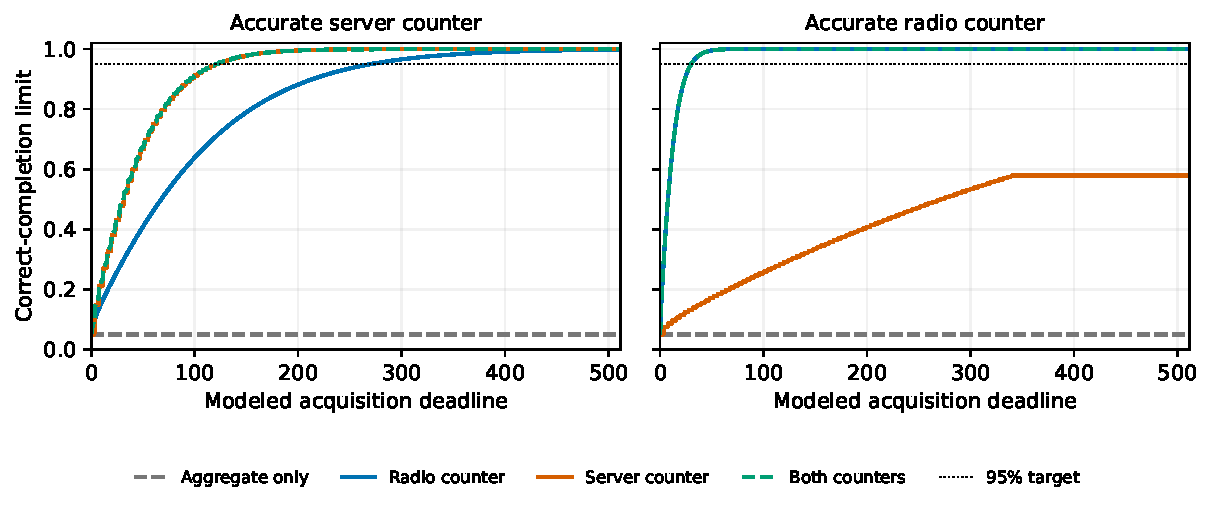
\includegraphics[width=\textwidth]{figures/v42_deadline_instrumentation_frontier.pdf}
\caption{Exact correct-completion limits at absolute stage margin $0.2$,
wrong-return risk $0.05$, and hard cost cap 512. Lines give the exact
reference. Counter precision changes
which instrumentation can meet a deadline. The aggregate-only line is a
randomized 5\% upper bound; our operational policies always abstain in
that case. Radio and both-counter curves coincide in the right panel.
Durations are modeled acquisition units.}
\label{fig:v42-scalar-frontier}
\end{figure*}

Across the 144 positive-information endpoint cells, the largest absolute
Monte Carlo discrepancy from exact completion is 1.545 percentage points;
the largest standardized discrepancy is 2.628. Independent replay checks
all scores and stopping decisions. The simulation is an implementation
check, not a proof of the frontier.

For the preselected $\vartheta=0.2$ case with both counters and the
accurate-server catalogue, deadline 128 gives 3919 correct and 177
unresolved endpoint returns out of 4096. Sequential execution gives 3877
correct, two wrong, and 217 unresolved returns, reducing mean all-attempt
cost from 192 to 164.883. Its observed completion is 94.65\%, compared
with 95.68\% for endpoint execution. At deadline 512, correct counts
are 4096 and 4094, with two sequential wrong returns and costs 512 and
294.700. Thus earlier decisions do not improve cost and completion
simultaneously in these cases. In the accurate-radio catalogue, the
corresponding endpoint/sequential correct counts are 4096/4093 at both
deadlines, with three sequential errors; costs are 128/52.176 and
512/52.413. All comparisons include unsuccessful attempts. Full
cellwise uncertainty and paired cost/completion differences remain in the
released tables.

\subsection{A Practical Controller with Both Counter Orientations}

We next retain the v41 six-mean finite-population model and its unchanged
joint verifier. Two complete radio-row relabelings exchange the fast and
slow stages, including configuration charges, bounds, report operators,
variance proxies, tape access, and goal constraints. Instrument access is
either all six probes or aggregates plus the fixed label-5 stage counter.
That restricted counter measures the fast stage in one orientation and the
other stage in the relabeled orientation. We do not choose the useful
counter separately for every condition.

We cross radio limits $3.8$ and $3.1$ ms, with total and server limits
$24$ and $8.5$ ms. Initial history is either empty or contains 256 reports
per aggregate probe. All new reports are charged; nonempty history costs
1920 sunk units. Every report still averages 64 independent virtual-task
draws from the frozen population. The count cap remains 4096 including
history, with error allocation $0.05$ and four-report online batches.
The simultaneous confidence bands, declared parameter box, and complete certificate
are unchanged from the preceding study.

Coverage chooses the available probe with the smallest absolute count,
breaking ties with a seeded uniform permutation independent of report noise.
The relabeling transforms that priority consistently. A simple goal-directed
rule instead selects the cheapest configuration not yet jointly excluded,
identifies its unresolved feasibility constraints, and chooses the probe
with the largest directional uncertainty reduction per modeled duration.
Its regularized information matrix is only an acquisition heuristic.
Regularization supplies no evidence and changes no authorization condition.
The score is a standard experimental-design heuristic, not a new statistical
guarantee or an optimal multidimensional controller.

Each policy follows one acquisition sequence, with checks initially and
after each complete batch. We evaluate its prefixes at duration limits
$0$, $16$, $32$, $64$, $128$, $256$, and $512$. The policy returns at its
first complete certificate, model conflict, cap exhaustion, or resource
limit. A counterfactual shorter execution stops before ordering a batch
that cannot finish in time. We include its acquisition cost and the selector
computation needed to make that stopping decision. The acquisition sequence
does not change with the deadline; these are achievable completion curves,
not optimal deadline-dependent policies.

Sixteen held-out seeds give 512 complete trial traces and 3584
policy/deadline outcomes. All orientations and deadline views of a seed
remain together when computing paired uncertainty. We report Wilson
completion intervals and 10,000 seed-cluster bootstrap replicates for paired
differences. The fixed goals, conditions, score, and analysis precede
evaluation. All initial integration attempts remain in the development
records.

Table~\ref{tab:v42-practical} reports every instrumentation, history,
and goal condition at the final deadline. All-instrument orientations have
identical outcomes under their complete paired relabeling. With empty
history and all instruments, goal-directed acquisition completes $16/16$
trials at deadline 512 for both goals; coverage remains unresolved in all.
With history and the $3.8$-ms goal, goal-directed acquisition completes
$16/16$ by deadline 64, whereas coverage first does so on the reported
grid at 128. With the $3.1$-ms goal, their counts at deadline 256 are
$15/16$ and $0/16$, and at 512 are $16/16$ and $15/16$.

\begin{table*}[t]
\centering
\caption{Practical completion and mean online acquisition cost at modeled
deadline 512. C denotes coverage and G the goal-directed heuristic.
Each row has 16 seeds; orientations are paired relabelings. Costs include
unresolved attempts. Unequal completion precludes interpreting the cost
ratio as equivalent-service savings. Nonempty history adds 1920 sunk units.}
\label{tab:v42-practical}
\small
\begin{tabular}{@{}ccclrrrr@{}}
\toprule
Orientation & History/probe & Radio limit & Instruments & C correct & G correct & C cost & G cost\\
\midrule
Both & 0 & 3.1 & All & 0/16 & 16/16 & 1615.10 & 1628.75\\
Both & 0 & 3.8 & All & 0/16 & 16/16 & 1615.10 & 1004.89\\
Both & 256 & 3.1 & All & 15/16 & 16/16 & 2517.00 & 1275.00\\
Both & 256 & 3.8 & All & 16/16 & 16/16 & 564.00 & 297.00\\
0 & 0 & 3.1 & Fixed 5 & 0/16 & 16/16 & 1248.00 & 1564.69\\
0 & 0 & 3.8 & Fixed 5 & 0/16 & 16/16 & 1248.00 & 974.63\\
0 & 256 & 3.1 & Fixed 5 & 16/16 & 16/16 & 1275.00 & 1275.00\\
0 & 256 & 3.8 & Fixed 5 & 16/16 & 16/16 & 297.00 & 297.00\\
1 & 0 & 3.1 & Fixed 5 & 0/16 & 0/16 & 1248.00 & 880.04\\
1 & 0 & 3.8 & Fixed 5 & 0/16 & 0/16 & 1248.00 & 918.77\\
1 & 256 & 3.1 & Fixed 5 & 0/16 & 0/16 & 3072.00 & 832.20\\
1 & 256 & 3.8 & Fixed 5 & 0/16 & 0/16 & 3072.00 & 832.20\\
\bottomrule
\end{tabular}
\end{table*}

The useful fixed counter with history makes both acquisition rules
identical: they complete the loose goal by 64 and the tighter goal by 512,
with $15/16$ tighter-goal completions at 256. The wrong fixed counter
leaves both rules unresolved at every reported deadline. A structural
construction below explains that condition; unresolved all-instrument
prefixes alone prove no impossibility.

Sixteen successes give a pointwise 95\% Wilson interval of
$[80.6,100]\%$; zero give $[0,19.4]\%$. Paired bootstrap intervals
can degenerate when every observed difference is identical and do not
establish population certainty. The full seven-deadline tables and
uncertainty estimates are released. These results compare simple policies
under a common verifier; they neither replace the separate 2.36\%
maximin comparison nor establish a new allocation algorithm. Different
response and noise models also prevent interpreting their distance from
the scalar reference as an optimality gap.

\subsection{An Obstruction with the Wrong Counter}

In original full-stage coordinates
$(r_0,r_1,w_{00},w_{01},w_{10},w_{11})$, the restricted orientation observes
all aggregate sums and only the slow radio $r_0$. Change the unobserved
radio and its two associated server stages by
$$v=(0,2,0,0,-2,-2).$$
Every available direction annihilates $v$. More strongly, adding these
constants to each component observation preserves every aggregate report
and the observed radio law. Support widths and independence are unchanged;
all full-stage observations remain nonnegative, with minimum 3.2 ms, and
all means remain inside the declared box. The base state requires
configuration 3; the changed state has no feasible configuration under
either radio goal. This is an analytical construction in the flexible
bounded-stage class, not another physical observation or sampled population.

The two acquired transcript laws are identical for any causal controller
using that access, including aggregate history. A valid answer in either
state is wrong in the other, so uniform wrong-return risk $\delta$ bounds
correct completion by $\delta$ at each state for every deadline. This
row-specific change, unlike the earlier global shift, preserves the exposed
counter. The argument permits radio-dependent server means; imposing known
server-row equality can remove the alternative. Its validity therefore
depends on the complete admitted prior, as the next sensitivity illustrates.

\subsection{Known Physical Priors Remove an Earlier Separation}
\label{app:prior-sensitivity}

A post-evaluation audit identifies a consequential prior-information issue.
The population generator adds nonnegative radio workload to known nominal
service times approximately $(3.88845,1.54168)$ ms. Both matched states
retain these lower bounds: the second adds a nonnegative two-ms radio shift.
However, the frozen six-mean verifier uses zero as each lower bound. That
broader box omits physical information available from this generator. In
particular, the slow radio's nominal service already exceeds both radio
limits, so its configurations can be excluded without measurement.

We replay every original one-fast-counter trace with only these two radio
lower bounds strengthened equally for both verifiers. We add no server
nominal lower bounds, because the constructed negative server shifts need
not preserve them. The recorded streams, aggregate history, coverage
allocation, goal, confidence bands, and original duration limits stay fixed.
This is an explicitly post-evaluation sensitivity using existing data,
not a newly preregistered confirmation or a new sampled experiment.

At both original duration limits (150 and 2000), both joint and componentwise
verification now complete $32/32$ trials in each matched state, at duration
64 and cost 384. Their earlier $32/32$ versus $0/32$ difference disappears
completely. In the unshifted state, the prior excludes the slow row;
fast-radio evidence then certifies the returned configuration and permits
componentwise server exclusion of its remaining cheaper rival. In the
shifted state, the observed fast-radio violation excludes the remaining
row. This does not invalidate the algebraic joint-separation
results; it removes this fixture's empirical advantage under stronger,
physically justified information.

The frozen practical curves above deliberately retain their original
zero-lower-bound model. They are internally reproducible under that declared
class, but cannot establish a physical advantage with all known priors
included. The release preserves the original study and the adverse
sensitivity separately. Claims about required instrumentation and benefits
over componentwise certification must state all valid physical bounds and
structural equalities supplied to every method.

\subsection{Physical Evidence: Available Records and Required Collection}

The source audit finds no raw EdgeDroid records, original trace fit and
split, localhost harness, or request/timestamp logs in the supplied release.
The earlier numerical summaries remain historical reports; they cannot
establish physical calibration, dependence control, or an evidence-validity
horizon. We execute no new physical experiment and recover no verified raw
dataset in this milestone.

The release supplies a concrete raw-record schema and executable preflight
for a crossed two-radio by two-server collection. Required fields identify
the configuration, context, epoch, collection block and split, workload,
terminal status, measurement meaning, timing units and clock domain.
Failures, timeouts, and unfinished work remain in the record ledger.
Within-clock elapsed durations are distinct from unsupported differences
between clocks. Subtracting server time from RTT yields a non-server
round-trip residual, not automatically one-way radio delay.

Eighteen scripted integrity cases pass, using explicitly synthetic example
records. The preflight reports that statistical validity is not established:
schema consistency does not demonstrate independent observations, accurate
clocks, a bounded response law, or future stability. Physical inference
still needs the original trace and metadata, or a new instrumented collection
with justified sampling units, independent calibration/evaluation blocks,
stage attribution, and measured acquisition, controller, and actuation times.

\balance
\subsection{Replay and Supported Interpretation}

The independent scalar replay passes all 1,966,080 raw outcomes,
24,624 exact-curve rows, 48 target boundaries, and 240 paired comparisons.
It independently enumerates legal integer designs and regenerates every
Gaussian tape and stopping decision. These checks do not treat the
correlated condition views as independent replications.

The practical replay passes 512 trial traces, 3584 deadline views,
372,312 raw reports, 28,054 reconstructed confidence prefixes, 286 exact
rational certificates, all 224 summary cells, and 112 paired comparisons.
There are 604 approved deadline views and no wrong returns; these repeated
views are not 604 independent successes. The auditor reconstructs public
metadata, relabelings, confidence bands, selector scores, risk accounting,
and terminal evidence independently of the acquisition controller.

The separate prior sensitivity passes 64 archived traces, 128 exact
rational certificates, and 256 deadline views. The first certifying prefix
coincides for both verifiers in every trace. The auditor also verifies that
the two incompatible matched states remain in each strengthened
history-only confidence set, ruling out an earlier certified answer there.
This gate verifies the adverse comparison on existing evidence; it supplies
no new physical validation.

The scalar experiment connects a proven resource limit to an executable
controller, under its stated Gaussian assumptions. The practical experiment
tests how a simple goal-derived rule behaves when history, margins, and
counter orientation change. Its unresolved outcomes do not establish the
optimal multidimensional frontier or a physical impossibility. The restricted wrong-counter condition has a separate identical-law
construction under its declared flexible model; failed prefixes with full
instrumentation have no such impossibility interpretation. These results justify distinct engineering
responses to missing information, insufficient acquisition time, and binding
cost caps while preserving the remaining physical-validation obligations.
The full protocols, code, outcomes, and auditors appear under
\texttt{research\_v42/}.
